%**************************************************************************
%*
%*  Instrucciones para la platilla del informe final
%*
%*  
%*
%*  Filename: platillapaper.tex
%*
%*
%*  
%*  
%*
%**************************************************************************


\documentclass{wscpaperproc}
\usepackage[spanish]{babel}
\usepackage{latexsym}
\usepackage{caption}
\usepackage{csquotes}
\usepackage{graphicx}
\usepackage{mathptmx}
\usepackage[T1]{fontenc}
\usepackage[style=numeric,backend=biber,defernumbers=true, sorting=none]{biblatex}
\addbibresource{EDO Final Work.bib}

%
%****************************************************************************
% AUTHOR: You may want to use some of these packages. (Optional)
\usepackage{amsmath}
\usepackage{amsfonts}
\usepackage{amssymb}
\usepackage{amsbsy}
\usepackage{amsthm}
\usepackage[colorlinks=true,urlcolor=blue,citecolor=black,anchorcolor=black,linkcolor=red]{hyperref}
\usepackage{hyperref}
%****************************************************************************


%
%****************************************************************************
% AUTHOR: If you do not wish to use hyperlinks, then just comment
% out the hyperref usepackage commands below.

%% This version of the command is used if you use pdflatex. In this case you
%% cannot use ps or eps files for graphics, but pdf, jpeg, png etc are fine.

%% The next versions of the hyperref command are used if you adopt the
%% outdated latex-dvips-ps2pdf route in generating your pdf file. In
%% this case you can use ps or eps files for graphics, but not pdf, jpeg, png etc.
%% However, the final pdf file should embed all fonts required which means that you have to use file
%% formats which can embed fonts. Please note that the final PDF file will not be generated on your computer!
%% If you are using WinEdt or PCTeX, then use the following. If you are using
%% Y&Y TeX then replace "dvips" with "dvipsone"

%%\usepackage[dvips,colorlinks=true,urlcolor=blue,citecolor=black,%
%% anchorcolor=black,linkcolor=black]{hyperref}
%****************************************************************************


%
%****************************************************************************
%*
%* AUTHOR: YOUR CALL!  Document-specific macros can come here.
%*
%****************************************************************************

% If you use theoremes
\newtheoremstyle{wsc}% hnamei
{3pt}% hSpace abovei
{3pt}% hSpace belowi
{}% hBody fonti
{}% hIndent amounti1
{\bf}% hTheorem head fontbf
{}% hPunctuation after theorem headi
{.5em}% hSpace after theorem headi2
{}% hTheorem head spec (can be left empty, meaning `normal')i

\theoremstyle{wsc}
\newtheorem{theorem}{Teorema}
\renewcommand{\thetheorem}{\arabic{theorem}}
\newtheorem{corollary}[theorem]{Corolario}
\renewcommand{\thecorollary}{\arabic{corollary}}
\newtheorem{definition}{Definici\'on}
\renewcommand{\thedefinition}{\arabic{definition}}


%#########################################################
%*
%*  The Document.
%*
\begin{document}

%***************************************************************************
% AUTHOR: AUTHOR NAMES GO HERE
% FORMAT AUTHORS NAMES Like: Author1, Author2 and Author3 (last names)
%
%		You need to change the author listing below!
%               Please list ALL authors using last name only, separate by a comma except
%               for the last author, separate with "and"
%
\WSCpagesetup{Machado, Toledo, Moreno, Concepci\'on, Navarro}

% AUTHOR: Enter the title, all letters in upper case
\title{Estabilidad y simulaci\'on num\'erica del sistema presa-depredador con respuestas funcionales de tipo II de Holling para presas adultas}

% AUTHOR: Enter the authors of the article, see end of the example document for further examples
\author{
	Daniel Machado \\[12pt]
	Grupo C211\\
	Ciencia de la Computaci\'on\\
	Facultad de Matem\'atica y Computaci\'on\\
	Universidad de La Habana. Cuba\\
	% Multiple authors are entered as follows.
	% You may also need to adjust the titlevbox size in the preamble - search for titlevboxsize
	\and
	Daniel Toledo\\[12pt]
	Grupo C211\\
	Ciencia de la Computaci\'on\\
	Facultad de Matem\'atica y Computaci\'on\\
	Universidad de La Habana. Cuba\\
	\and
	Osvaldo Moreno\\[12pt]
	Grupo C211\\
	Ciencia de la Computaci\'on\\
	Facultad de Matem\'atica y Computaci\'on\\
	Universidad de La Habana. Cuba\\
	\and
	Jos\'e Antonio Concepci\'on\\[12pt]
	Grupo C211\\
	Ciencia de la Computaci\'on\\
	Facultad de Matem\'atica y Computaci\'on\\
	Universidad de La Habana. Cuba\\
	\and
	Adri\'an Navarro\\[12pt]
	Grupo C211\\
	Ciencia de la Computaci\'on\\
	Facultad de Matem\'atica y Computaci\'on\\
	Universidad de La Habana. Cuba\\
}



\maketitle

\section*{Resumen}
Este documento presenta un análisis local exhaustivo del modelo depredador-presa con estructura de
etapas en la población de presa y respuestas funcionales de Holling de tipo II y I \cite{holling_functional_1965}. Los autores determinan
los tres posibles equilibrios, analizan la estabilidad local a través de la matriz jacobiana, realizan
simulaciones numéricas y obtienen varios resultados clave. El equilibrio trivial siempre es inestable,
el equilibrio con predadores extintos es estable bajo ciertas condiciones y el equilibrio interior puede
ser estable o inestable dependiendo de los parámetros. Las simulaciones numéricas corroboran estos resultados
y muestran cómo las poblaciones evolucionan hacia uno de los tres puntos de equilibrio dependiendo de las
condiciones iniciales y los valores de parámetros.

\section{INTRODUCCI\'ON}
\label{sec:intro}
El artículo titulado "Local Analysis of the Prey-Predator Model with Stage-Structure Prey and Holling
Type Functional Responses" por Dian Savitri fue publicado en 2019
en el Journal of Physics: Conference Series. Su factor de impacto tiene una puntuaci\'on de 0.21 en el
período 2022-2023. El artículo analiza el modelo depredador-presa con dos tipos de presa en estructura
de etapas y un solo depredador. La población de presas se divide en adultos y juveniles. El depredador
exhibe diferentes tasas de depredación para adultos e inmaduros. Se utilizan respuestas funcionales de
Holling tipo II \cite{holling_functional_1965} para adultos y tipo I para juveniles. El estudio tuvo los siguientes objetivos:
determinar los puntos de equilibrio del modelo, analizar la estabilidad local de los puntos de equilibrio
utilizando la matriz jacobiana y autovalores y observar el comportamiento dinámico del modelo mediante
simulaciones numéricas y diagramas de fase. Además utilizaron las siguientes técnicas para obtener resultados
más rigurosos: análisis matemático para determinar los puntos de equilibrio y condiciones de estabilidad,
cálculo de la matriz jacobiana y autovalores en cada punto de equilibrio, aplicación del Criterio de Routh-Hurwitz
para analizar la estabilidad del equilibrio interior, simulaciones numéricas utilizando el método Runge-Kutta de
cuarto orden y un análisis de bifurcación para estudiar la posible existencia de ciclos límite. (no estoy seguro de esta traduccion revisar despues)

\section{Modelo Propuesto}

El artículo analiza previamente tres modelos matemáticos que abordan las interacciones presa-depredador con diferentes enfoques. El 
primer modelo propuesto por Huenchucona considera dos presas y un depredador, utilizando una 
función de respuesta de tipo Beddington-DeAngelis \cite{falconi_stability_2015}. El modelo de Savitri y Abadi tiene en cuenta la estructura 
por etapas de la presa, utilizando funciones de respuesta diferentes para presas inmaduras y maduras \cite{savitri_dynamics_2018}. Luego, el 
modelo de Castellanos y Chan-López estudia una cadena trófica de tres niveles, donde la presencia del depredador 
superior afecta la estabilidad del sistema \cite{castellanos_existence_2017}. Los sistemas de ecuaciones de dichos modelos (\ref{twoPreyonePredator_Falconi}, \ref{Holling1y2_Abadi}, 
\ref{Holling1y2_Castellanos} respectivamente) pueden ser consultadas en los Anexos \ref{app:Anexos}.\par

Estos modelos constituyen una base para el análisis 
del sistema propuesto que está dado por los siguientes sistemas de ecuaciones diferenciales donde se definen \emph{x(t)}, \emph{y(t)} y \emph{z(t)} como la 
densidad de la poblaci\'on de presas j\'ovenes, presas adultas y depredadores respectivamente.
La primera ecuación describe las presas juveniles crece con la tasa de crecimiento intrínseca \emph{r} haciendo que aumente la tasa de crecimiento de la población de 
presas juveniles. La tasa de depredación para ambas poblaciones de presas es diferente. Se asume que el depredador puede asechar 
tanto a las presas juveniles como a las presas adultas en el modelo estructurado. La tasa de depredación del depredador utiliza el Holling tipo II
para la especie de presa adulta y el Holling tipo I para la presa juvenil. La tasa de depredación se da en la forma original de la respuesta funcional 
de tipo II de Holling, donde $\eta$  y \emph{m} son el valor máximo de la tasa de reducción per cápita de \emph{y} debido a \emph{z} y el coeficiente 
de protección ambiental para la presa adulta, respectivamente. La tasa de cambio en las densidades de población de presas juveniles por las tasas de crecimiento intrínsecas se 
reducen por la tasa a la que las presas juveniles son consumidas por los depredadores. Las poblaciones de presas juveniles crecen con ecuaciones logísticas 
que se ven limitadas por la capacidad de carga \emph{(k)} para mantener sus poblaciones.\par

\begin{equation} \label{twoPreyonePredatorEDO}
	\begin{gathered}
		\frac{d x}{d t}=r x\left(1-\frac{x}{k}\right)-\beta x-\alpha x z \\
		\frac{d y}{d t}=\beta x-\frac{\eta y z}{y+m}-\mu y \\
		\frac{d z}{d t}=\alpha_1 x z+\rho z^2-\frac{\eta_1 y z}{y+m}
	\end{gathered}
\end{equation}
\par
El índice de depredación de presas juveniles es proporcional a la tasa a la cual los depredadores 
y las presas juveniles se encuentran, también conocido como la ecuación de Lotka-Volterra. Los parámetros $r, \beta, \alpha, \alpha, \rho, m, \mu, \nu, \alpha_1, \nu_1$ son positivos. 
Los cambios en la densidad de población de las presas adultas representan el crecimiento de las presas adultas debido al factor de conversión de presas 
juveniles a presas adultas. 
El parámetro $\eta$ en el proceso de depredación provoca una disminución en la población de presas adultas, lo que se interpreta 
como la tasa de encuentros con presas adultas por unidad de densidad de presas adultas. Sin depredación, las presas adultas experimentan un proceso natural 
de muerte. La tasa de depredación de los depredadores sigue la respuesta funcional del tipo II de Holling. La relación $\frac{m}{\nu}$ es el tiempo promedio de 
procesamiento de alimentos para el depredador. El parámetro $\rho$ es la tasa de crecimiento de la población de depredadores. Se asume que la tasa de cambio 
en la población de depredadores disminuye siguiendo el modelo de Leslie-Gower {citar}, donde \emph{m} representa la pérdida de residuos de depredadores debido a la 
falta de su alimento favorito. El parámetro $\eta_1$ es la relación del crecimiento intrínseco dividido por el factor de conversión de depredación a presas adultas. 
Esto afecta la disponibilidad de alimentos favoritos por individuo, que está determinada por la capacidad de los recursos ambientales y es proporcional a la 
abundancia de sus alimentos favoritos.

\subsection{M\'etodos y algoritmos utilizados}
Esta  subsecci\'on se describen los c\'odigos de programas utilizados en el trabajo mediante las siguiente instrucciones.

\begin{verbatim}
y_{n+1}=y_n+hf(x_n,y_n}
\end{verbatim}


\begin{itemize}
	\item Utilice vi\~netas est\'andar en lugar de tildes, flechas, etc.
\end{itemize}
\begin{enumerate}
	\item En las listas numeradas, las etiquetas no deben ser n\'umeros ar\'abigos encerrados entre par\'entesis,
\end{enumerate}


\begin{table}[htb]
	\centering
	\caption{Uso de tabla\label{tab: first}}
	\begin{tabular}{rll}
		\hline
		- & IQ & Dieta          \\ \hline
		- & 70 & Cualquier cosa \\
		- & 60 & -              \\
		\hline
	\end{tabular}
\end{table}


% esto estaba en la plnatilla no tocar por ahora()
% \begin{figure}[htb]
% {
% \centering
% 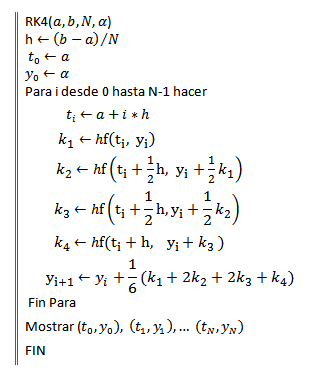
\includegraphics[width=0.50\textwidth]{alg_rk4}
% \caption{Figura-I.\label{fig: tahi}}
% }
% \end{figure}

.
\begin{definition}

\end{definition}

\begin{theorem}

\end{theorem}

\begin{corollary}
	aslkjdfkl;asjdfk;ljasd;lkfjal;ksjgklasjkgajsf
\end{corollary}

% no tocar por si hace falta despues pero esta bien feo
% {\footnotesize
% \begin{hangref}
% \item Banks, J., J. S. Carson, B. L. Nelson, and D. M. Nicol. 2000. \textit{Discrete-Event System Simulation}. 3rd ed. Upper Saddle River, New Jersey: Prentice-Hall, Inc.
% \end{hangref}
% }

\section*{Conclusiones}
Este estudio proporciona una comprensi\'on más profunda de las complejas interacciones entre los depredadores y sus presas en
los ecosistemas naturales. Los resultados obtenidos pueden ser \'utiles para predecir y manejar las poblaciones de presas y
depredadores en diferentes entornos y para comprender mejor los efectos del cambio clim\'atico y otros factores ambientales
en estas interacciones. FALTA Añadir una valoración de lo que usted ha aprendido con este trabajo, como valora la
posibilidad de que se pueda continuar esta línea de investigación.

\section*{F\'ORMULAS A UTILIZAR DESPU\'ES}
% aqui ya estan la mayoria de las formulas

\begin{equation} \label{JacobianoEstability}
	J\left(x^*, y^*, z^*\right)=\left[\begin{array}{ccc}
			\mathrm{r}-\frac{2 r x}{k}-\beta-\alpha z & 0                                                                  & -\alpha x                                        \\
			\beta                                     & -\frac{\eta \mathrm{z}}{y+m}+\frac{\eta y \mathrm{z}}{(y+m)^2}-\mu & -\frac{\eta \mathrm{y}}{y+m}                     \\
			\alpha_1 z                                & \frac{\eta_1 \mathrm{z}^2}{(y+m)^2}                                & 2 p z-\frac{2 \eta_1 \mathrm{z}}{y+m}+\alpha_1 x
		\end{array}\right]
\end{equation}

\begin{equation} \label{Characteristic000}
	\left|\begin{array}{ccc}
		(-1+r)-\lambda & 0            & 0         \\
		\beta          & -\mu-\lambda & 0         \\
		0              & 0            & 0-\lambda
	\end{array}\right|=0
\end{equation}

\begin{equation} \label{Equilibrium}
	\begin{aligned}
		 & \operatorname{det}\left(J\left(\frac{k(r-\beta)}{r}, \frac{\beta k(r-\beta)}{\mu r}, 0\right)-\lambda I\right)=0                            \\
		 & J\left(E_2\right)=\left|\begin{array}{ccc}
			                           (\beta-r)-\lambda & 0            & \frac{\alpha k(\beta-r)}{r}                                                      \\
			                           \beta             & -\mu-\lambda & \frac{\eta \beta k(\beta-r)}{r \mu\left(\frac{\beta k(r-\beta)}{\mu r}+m\right)} \\
			                           0                 & 0            & -\frac{\alpha_1 k(\beta-r)}{r}
		                           \end{array}\right|=0
	\end{aligned}
\end{equation}

\begin{equation} \label{CharacteristicPolynomial}
	J\left(x^*, y^*, z^*\right)=\left[\begin{array}{ccc}
			\mathrm{r}-\frac{2 r x^*}{k}-\beta-\alpha z^* & 0                                                                   & -\alpha x^*                                     \\
			\beta                                         & -\frac{\eta z^*}{y^*+m}+\frac{\eta y z^*}{\left(y^*+m\right)^2}-\mu & -\frac{\eta y^*}{y^*+m}                         \\
			\alpha_1 z^*                                  & \frac{\eta_1 z^{* 2}}{\left(y^*+m\right)^2}                         & 2 p z^*-\frac{2 \eta_1 z^*}{y^*+m}+\alpha_1 x^*
		\end{array}\right]
\end{equation}

\defbibheading{Referencias}{\section*{Referencias}}
\defbibheading{Bibliografía}{\section*{Bibliografía}}

\printbibliography[heading=Referencias, type=article]
\renewcommand{\theenumiv}{}
\DeclareFieldFormat{labelnumberwidth}{}
\printbibliography[heading=Bibliografía, type=book, resetnumbers=true]
\nocite{edwards_differential_2008}



\section*{Agradeciemientos}
Agradecemos a nuestros queridos profesores por lograr que entendieramos de que van las ecuaciones diferenciales :D

\appendix

\section{Anexos} \label{app:Anexos}

\begin{center}
	Modelo propuesto por Huenchucona, Falconi y Vidal
	\\
\end{center}

\begin{equation} \label{twoPreyonePredator_Falconi}
	\begin{gathered}
		\frac{d x_1}{d t}=r x_1\left(1-\frac{x_1}{K}\right)-\beta x_1-\frac{\beta_1 x_1 y}{1+m_1 x_1^2+n_1 x_2} \\
		\frac{d x_2}{d t}=\beta x_1-\frac{\beta_2 x_2 y}{1+m_2 x_1+n_2 x_2}-\mu_1 x_2                           \\
		\frac{d y}{d t}=\frac{\alpha_1 \beta_1 x_1 y}{1+m_1 x_1^2+n_1 x_2}+\frac{\alpha_2 \beta_2 x_2 y}{1+m_2 x_1+n_2 x_2}-\mu_2 y
	\end{gathered}
\end{equation}
\\
\begin{center}
	Modelo propuesto por Savitri y Abadi
	\\
\end{center}
\begin{equation} \label{Holling1y2_Abadi}
	\begin{gathered}
		\frac{d x_1}{d t}=r x_1\left(1-\frac{x_1}{K}\right)-\beta x_1-\alpha x_1 y \\
		\frac{d x_2}{d t}=\beta x_1-\frac{\varepsilon x_2 y}{1+m x_2}-\mu_1 x_2 \\
		\frac{d y}{d t}=\frac{\gamma \varepsilon x_2 y}{1+m x_2}-\mu_2 y
	\end{gathered}
\end{equation}

\begin{center}
	Modelo propuesto por Castellanos y Chan-López
\end{center}
\begin{equation} \label{Holling1y2_Castellanos}
	\begin{gathered}
		\frac{d x}{d t}=\rho x\left(1-\frac{x}{k}\right)-a_1 x \\
		\frac{d y}{d t}=c a_1 x y-d y-\frac{a_2 y z}{y+b_2} \\
		\frac{d z}{d t}=\alpha z^2-\frac{\beta z^2}{y+b_2}
	\end{gathered}
\end{equation}


\begin{equation} \label{eq:quadraticsol}
	x = \frac{-b \pm \sqrt{b^2-4ac}}{2a} \mbox{ si } a \ne 0.
\end{equation}

\end{document}

